\documentclass[conference]{IEEEtran}
\IEEEoverridecommandlockouts
\usepackage{cite}
\usepackage{amsmath,amssymb,amsfonts}
\usepackage{algorithmic}
\usepackage{graphicx}
\usepackage{textcomp}
\usepackage{xcolor}
\usepackage{booktabs}
\usepackage{multirow}
\usepackage[hidelinks]{hyperref}

\def\BibTeX{{\rm B\kern-.05em{\sc i\kern-.025em b}\kern-.08em
    T\kern-.1667em\lower.7ex\hbox{E}\kern-.125emX}}

\begin{document}

\title{Leakage-Governed Medical Insurance Claim Fraud Detection Using Classical Ensembles, Tabular Deep Learning, and Dual-Path Agentic Triage}

\author{\IEEEauthorblockN{1\textsuperscript{st} B. Varshith}
\IEEEauthorblockA{\textit{Dept. of CSE (Data Science \& AI)} \\
\textit{IIIT Dharwad}, India \\
23bds011@iiitdwd.ac.in}
\and
\IEEEauthorblockN{2\textsuperscript{nd} J. Ganesh Kumar Reddy}
\IEEEauthorblockA{\textit{Dept. of CSE (Data Science \& AI)} \\
\textit{IIIT Dharwad}, India \\
23bds024@iiitdwd.ac.in}
\and
\IEEEauthorblockN{3\textsuperscript{rd} M. Jagadeeswar}
\IEEEauthorblockA{\textit{Dept. of CSE (Data Science \& AI)} \\
\textit{IIIT Dharwad}, India \\
23bds033@iiitdwd.ac.in}
\and
\IEEEauthorblockN{4\textsuperscript{th} Ramesh Athe}
\IEEEauthorblockA{\textit{Dept. of Computer Science \& Eng.} \\
\textit{IIIT Dharwad}, India \\
Project Supervisor}
}

\maketitle

\begin{abstract}
Medical insurance fraud screening suffers when black-box classifiers exploit upstream data leakage, rely on single-feature shortcuts, or lack deployable explainability for investigators. We present a comprehensive benchmark, leakage-governance protocol, and dual-path engineering platform evaluated across 4,500 medical insurance claims (6.00\% fraud prevalence). Our study unites three complementary paradigms: five Classical Machine Learning algorithms, five PyTorch Deep Learning models (\texttt{MLP}, \texttt{ResidualMLP}, \texttt{CNN1D}, \texttt{TabTransformer}, and an unsupervised \texttt{Autoencoder}), and an Agentic AI and Explainability layer powered by Google Gemini 2.0 Flash. Auditing the source corpus uncovered two hidden structural traps: an upstream \texttt{Cluster} field concentrating 98.89\% of frauds (267/270) in Cluster 1, and an amount boundary excluding all frauds below \$7,465.07. Across a 32-run ablation matrix spanning \texttt{Baseline (29f)}, \texttt{Intake (28f, no Cluster)}, \texttt{No-Amount (27f)}, and \texttt{Temporal Intake} ($\ge$ 2024-03-11), tree ensembles demonstrate superior robustness: without \texttt{Cluster}, Random Forest achieves 1.0000 test PR-AUC and 0.9873 $F_1$ (0 false positives, bootstrap 95\% CI [0.9610, 1.0000]), preserving 1.0000 $F_1$ under strict chronological split, while linear and neural models degrade by 6.6--10.7 PR-AUC points. Removing \texttt{ClaimAmount} collapses all eight supervised models to 0.1869--0.2404 PR-AUC, quantifying single-variable reliance honestly. In the 29-feature full-stack contract, \texttt{TabTransformer} leads supervised neural models (0.9911 PR-AUC), while a legitimate-only Autoencoder yields a documented negative result (0.0523 PR-AUC, 0.0299 $F_1$) due to covariate manifold overlap. Finally, pure-JavaScript browser weight exports match Python reference scoring across 10,800 evaluations within $4.42 \times 10^{-7}$ maximum error and zero decision flips, deployed alongside a live three-tier React/Node/FastAPI application.
\end{abstract}

\begin{IEEEkeywords}
Healthcare Insurance Fraud Detection, Data Leakage, Shortcut Learning, Random Forest, TabTransformer, Precision-Recall AUC, Agentic AI, Explainable AI.
\end{IEEEkeywords}

\section{Introduction}
Automated medical insurance fraud detection requires separating anomalous billing behavior from routine clinical variance under severe positive-class scarcity (typically 1--10\% prevalence) \cite{dupreez2025fraud, bauder2017medicare}. Prior studies frequently compare a narrow set of classifiers on random cross-sectional splits while overlooking two failure modes: upstream target-proxy leakage \cite{kaufman2012leakage} and single-attribute shortcut reliance \cite{geirhos2020shortcut}.

To address both modeling accuracy and experimental rigor, this paper evaluates an end-to-end fraud intelligence platform built across three technical approaches:
\begin{enumerate}
    \item \textbf{Approach 1 (Classical Ensembles \& Kernel Baselines):} Logistic Regression, Random Forest \cite{breiman2001random}, XGBoost \cite{chen2016xgboost}, RBF SVM \cite{cortes1995support}, and HistGradientBoosting \cite{ke2017lightgbm}.
    \item \textbf{Approach 2 (Supervised \& Unsupervised Deep Learning):} Tabular MLP, ResidualMLP \cite{he2016deep, gorishniy2021revisiting}, 1D-CNN, attention-based \texttt{TabTransformer} \cite{huang2020tabtransformer}, and a legitimate-only reconstruction \texttt{Autoencoder} \cite{sakurada2014anomaly}.
    \item \textbf{Approach 3 (Agentic Triage, XAI & Co-Pilot):} Multi-stage React UI, Express \texttt{AgenticEnsemble-v1} handler, cryptographic SHA-256 XAI audit utility, and Gemini 2.0 Flash interactive claim co-pilot.
\end{enumerate}

Our contributions are fourfold: (i) uncovering \texttt{Cluster} proxy leakage and \texttt{ClaimAmount} boundary dependence via four controlled experimental contracts (\texttt{Baseline}, \texttt{Intake}, \texttt{No-Amount}, and \texttt{Temporal}); (ii) benchmarking 10 heterogeneous ML/DL models including an empirical negative Autoencoder ablation; (iii) enforcing imbalance-appropriate PR-AUC ranking and validation-only threshold selection with 1,000-replicate bootstrap confidence intervals; and (iv) verifying exact Python-to-Browser numerical parity ($4.42 \times 10^{-7}$ max error across 10,800 scores) alongside a live React/Node/FastAPI application.

\section{Related Work}
A recent systematic review of 137 healthcare fraud studies by du Preez et al.\ \cite{dupreez2025fraud} highlights tree ensembles as top performers on structured claim records while exposing widespread omission of temporal testing and audit-cost calibration. Bauder and Khoshgoftaar \cite{bauder2017medicare} and Johnson and Khoshgoftaar \cite{johnson2019medicare} evaluated Medicare claims under extreme skew, demonstrating the necessity of class-weighted training alternatives over naive majority accuracy (alongside synthetic oversampling techniques such as SMOTE \cite{chawla2002smote}).

In general tabular learning, Huang et al.\ \cite{huang2020tabtransformer} introduced \texttt{TabTransformer} to contextualize discrete attributes via self-attention, and Gorishniy et al.\ \cite{gorishniy2021revisiting} formalized tabular Residual MLPs. Yet Grinsztajn et al.\ \cite{grinsztajn2022tree} proved across 45 datasets that orthogonal tree splits retain structural advantages over neural networks under sharp threshold boundaries and uninformative features. Under heavy class imbalance, Saito and Rehmsmeier \cite{saito2015precision} showed Precision-Recall AUC dominates ROC-AUC, while Kaufman et al.\ \cite{kaufman2012leakage} and Geirhos et al.\ \cite{geirhos2020shortcut} established formal criteria for leakage and shortcut detection. Finally, cryptographic claim trails \cite{kapadiya2022blockchain}, SHAP attributions \cite{lundberg2017unified}, and Retrieval-Augmented Generation \cite{lewis2020retrieval} motivate human-in-the-loop agentic investigation platforms.

\section{Dataset Audit and Problem Formulation}

\subsection{Corpus Characteristics and Leakage Findings}
The immutable source workbook (\texttt{Health Insurance Fraud Claims.xlsx}, SHA-256 verified) holds $N = 4,500$ claims across 19 columns spanning 731 days (\texttt{2022-07-09} to \texttt{2024-07-08}) with zero missing or duplicate entries. Only 270 claims (6.00\%) are fraudulent ($y_i = 1$). Six near-unique identifiers (\texttt{ClaimID}, \texttt{PatientID}, \texttt{ProviderID}, \texttt{DiagnosisCode}, \texttt{ProcedureCode}, \texttt{ProviderLocation}; 3,876--4,500 unique values) are excluded from supervised matrices.

\begin{figure}[t]
\centering
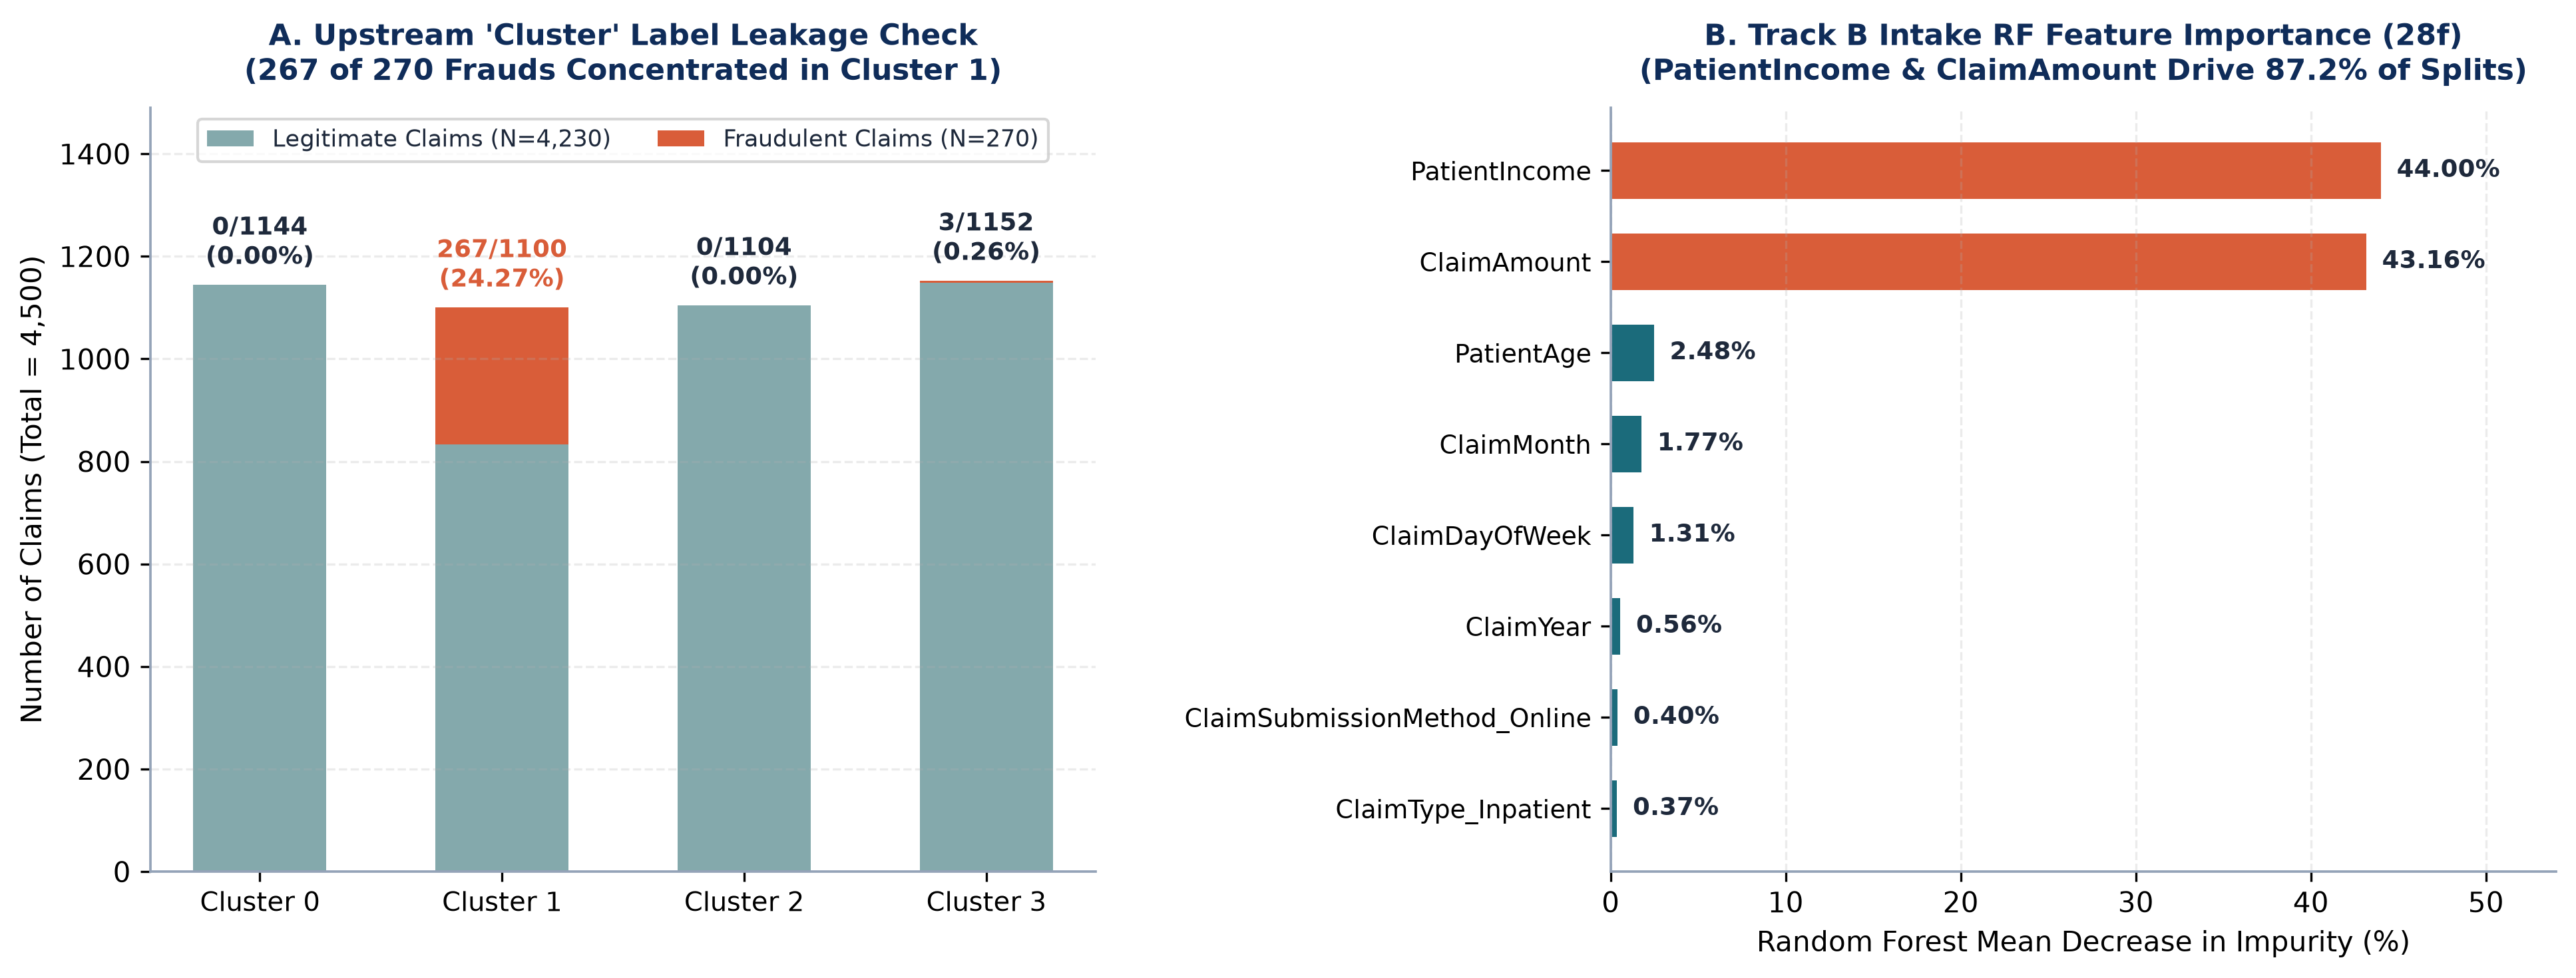
\includegraphics[width=\columnwidth]{figures/fig2_data_audit_shortcuts.png}
\caption{Audited distributional risks: (A) upstream \texttt{Cluster} concentrates 98.89\% of frauds in Cluster 1; (B) removing \texttt{Cluster} pushes Random Forest split importance onto \texttt{PatientIncome} (44.00\%) and \texttt{ClaimAmount} (43.16\%).}
\label{fig:audit}
\end{figure}

Exploratory cross-tabulation (Fig.~\ref{fig:audit}) revealed two critical properties: (1) upstream \texttt{Cluster} $\in \{0,1,2,3\}$ isolates 267/270 frauds (98.89\%) in Cluster 1 (24.27\% positive rate vs.\ 0.00\% in Clusters 0/2 and 0.26\% in Cluster 3); (2) \texttt{ClaimAmount} for frauds sits strictly in $[7,465.07, 9,978.43]$ (mean $8,733.57$), whereas legitimate claims span $[100.12, 9,997.20]$ (mean $4,776.80$).

\subsection{Experimental Contracts and Training Objectives}
We decouple backward compatibility from scientific ablation using two synchronized tracks:
\begin{itemize}
    \item \textbf{Track A (29 Features, 10 Models):} Stratified 70/15/15 split (Train 3,150 [189], Val 675 [41], Test 675 [40], seed 42) retaining \texttt{Cluster} to align all 5 Classical ML and 5 DL checkpoints behind Express and FastAPI.
    \item \textbf{Track B (4 Protocols $\times$ 8 Models = 32 Runs):}
    (i) \texttt{Baseline (29f)}, (ii) \texttt{Intake (28f, excluding Cluster)}, (iii) \texttt{No-Amount (27f, excluding Cluster and ClaimAmount)}, and (iv) \texttt{Temporal Intake} (Train $\le$ \texttt{2023-11-21} [3,152, 199], Val $\le$ \texttt{2024-03-10} [677, 34], Test $\ge$ \texttt{2024-03-11} [671, 37]).
\end{itemize}

All preprocessing scalers and one-hot encoders fit exclusively on $\mathcal{D}_{\text{train}}$. Supervised DL optimizes class-weighted binary cross-entropy:
\begin{equation}
\mathcal{L}_{\text{wBCE}}(\theta) = -\frac{1}{N_{\text{tr}}} \sum_{i=1}^{N_{\text{tr}}} \left[ w^+ y_i \log \sigma(z_i) + (1 - y_i)\log(1 - \sigma(z_i)) \right],
\end{equation}
where $w^+ = N_{-,\text{tr}} / N_{+,\text{tr}} \approx 15.67$. Conversely, the unsupervised \texttt{Autoencoder} minimizes reconstruction MSE on $y=0$ training samples with threshold set at the 95th validation percentile ($\tau_{\text{AE}} = 0.128588$). In Track B, operating thresholds $\tau^*$ maximize validation $F_1$ and remain frozen on test evaluation.

\section{Proposed Multi-Paradigm System Architecture}
Figure~\ref{fig:arch} summarizes the complete dual-path architecture connecting Approaches 1--3. Path A orchestrates a three-tier microservice stack: a React 19 + TypeScript UI (\texttt{:5173}), an Express API gateway (\texttt{:3000}) providing ML/DL proxying, deterministic \texttt{AgenticEnsemble-v1} four-event traces (\texttt{/agentic/predict}), and Google Gemini 2.0 Flash chat (\texttt{/api/chat}), plus a unified FastAPI + PyTorch/scikit-learn server (\texttt{:8000}) exposing all 10 checkpoints. Path B (\texttt{submission/}) compiles preprocessing scalers, linear coefficients, tree split rules, RBF dual coefficients, and PyTorch weight matrices directly to static JSON for client-side JavaScript inference (\texttt{:8080}). Meanwhile, Fig.~\ref{fig:agentic} documents Approach 3's honest engineering state, delineating verified Express/Gemini endpoints from the 6-agent frontend cards, SHA-256 \texttt{XAIExplainer} scaffold, and future live-model/RAG integration.

\begin{figure*}[t]
\centering
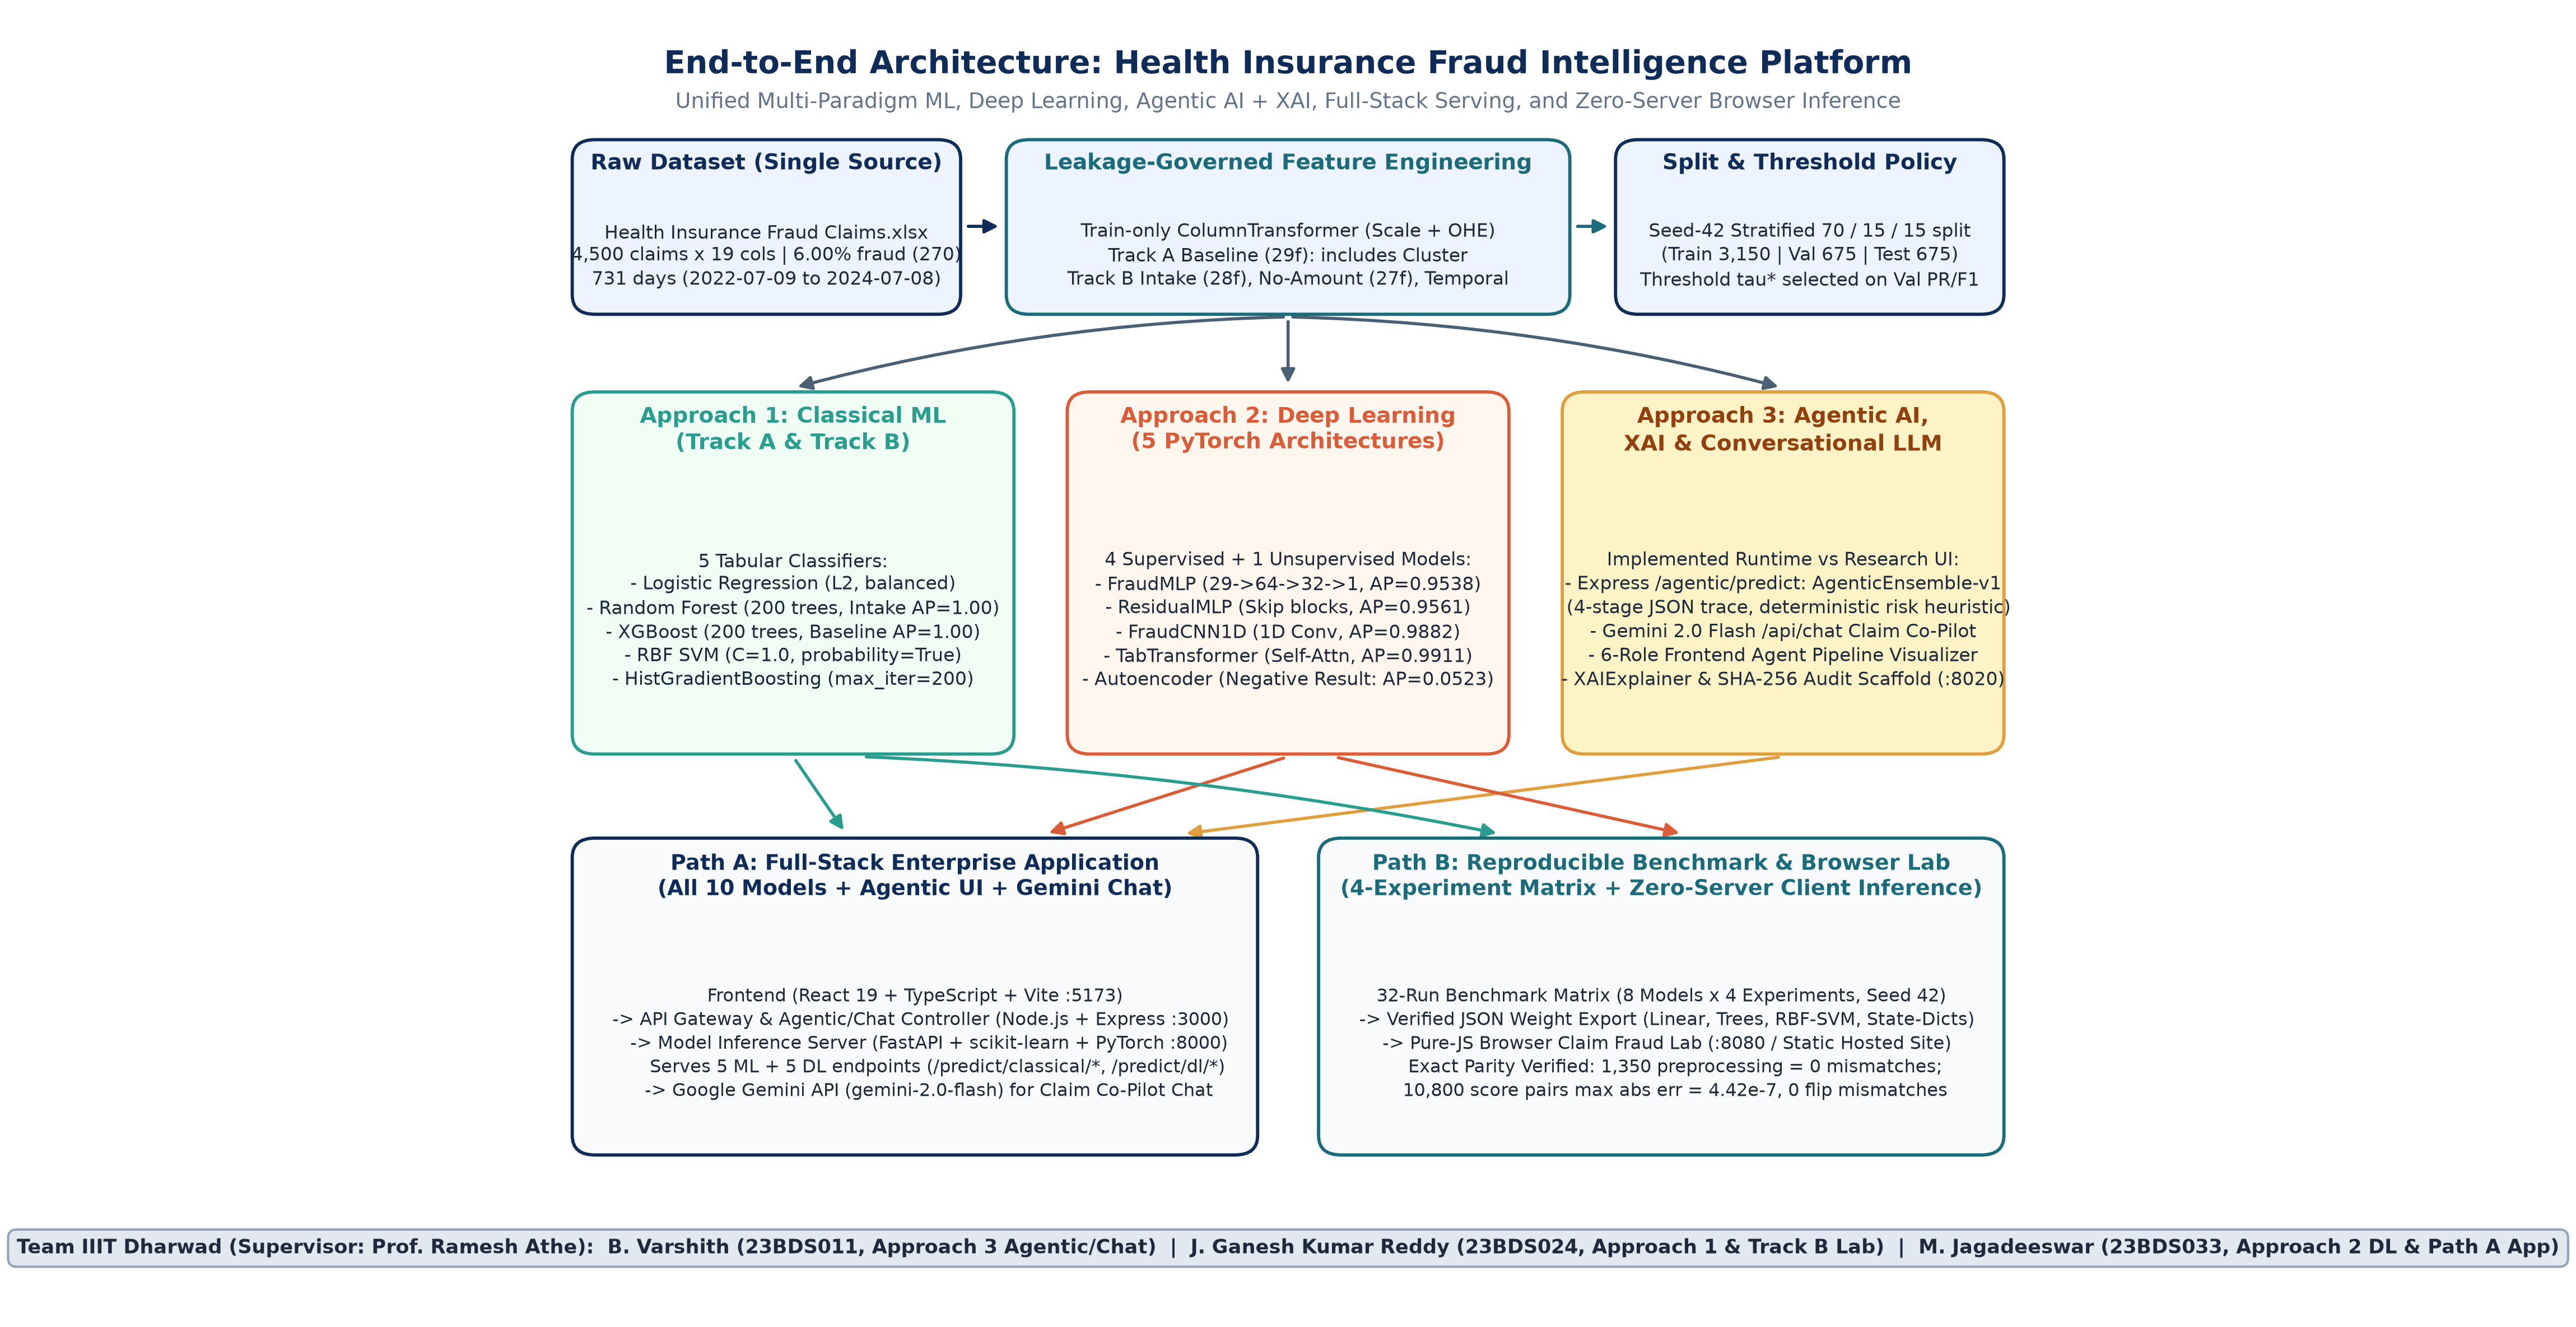
\includegraphics[width=0.92\textwidth]{figures/fig1_system_architecture.png}
\caption{End-to-end dual-path architecture integrating Approaches 1--3, the 3-tier React/Node/FastAPI web platform (Path A), and zero-server Claim Fraud Lab (Path B).}
\label{fig:arch}
\end{figure*}

\begin{figure}[t]
\centering
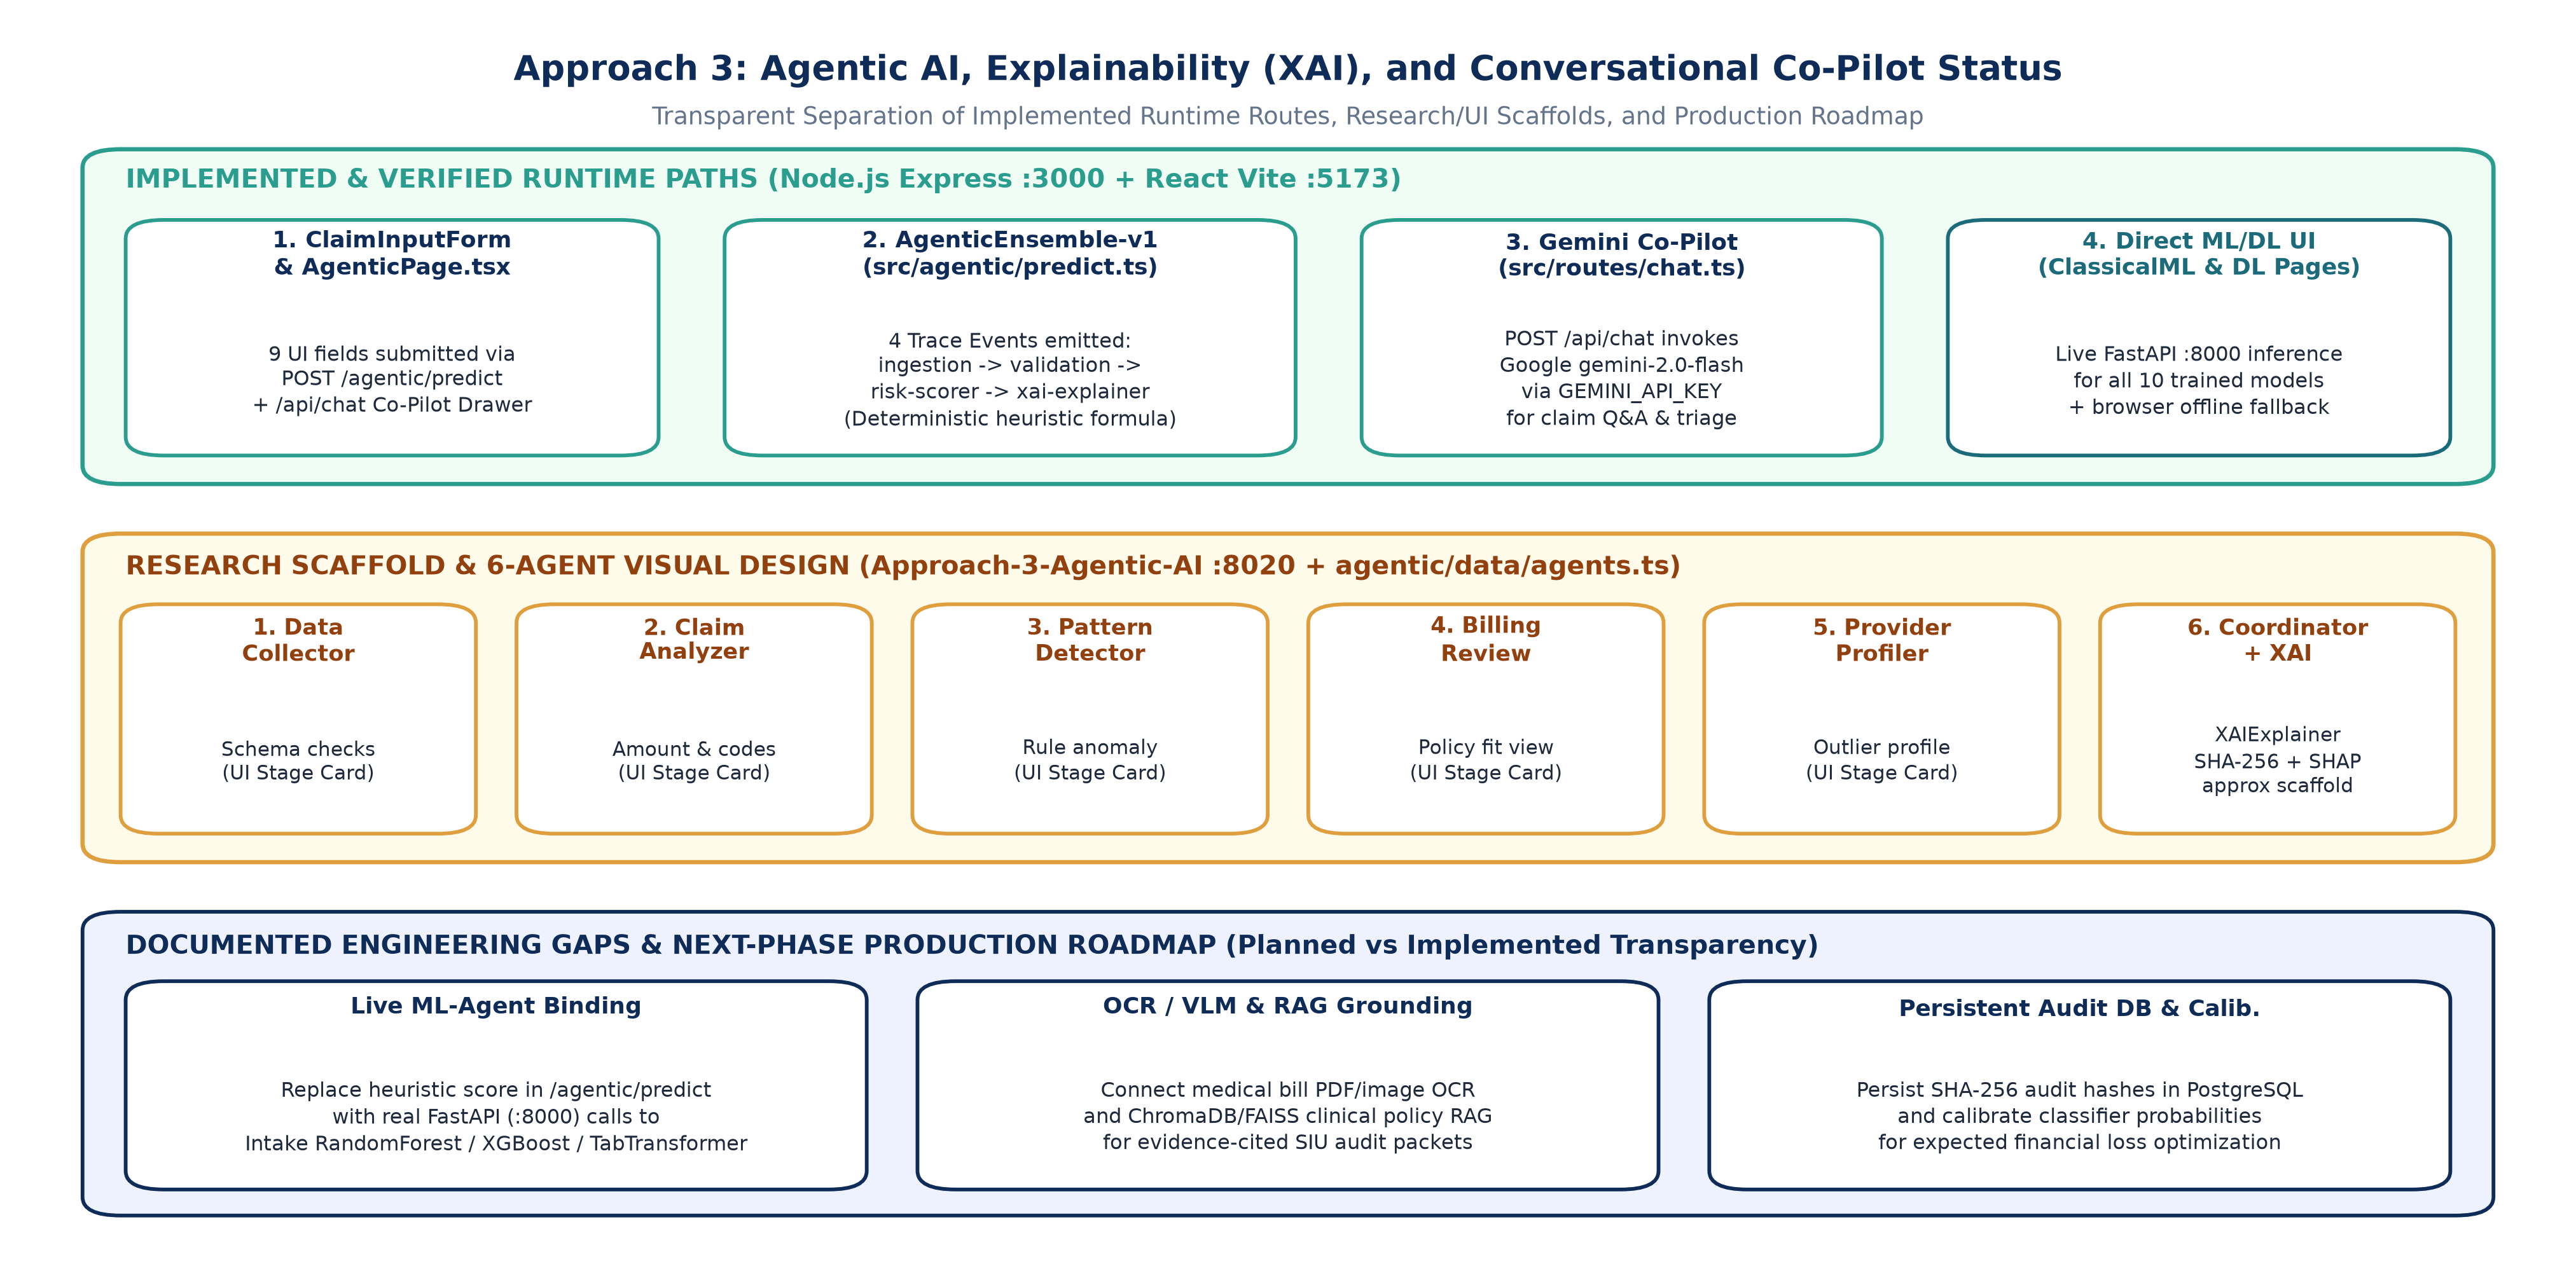
\includegraphics[width=\columnwidth]{figures/fig5_agentic_pipeline_status.png}
\caption{Approach 3 status separating implemented Express/Gemini runtime routes from the 6-role UI design and \texttt{XAIExplainer} scaffold.}
\label{fig:agentic}
\end{figure}

\section{Experimental Results and Verification}

\subsection{Track A: 10-Model Evaluation and Autoencoder Negative Study}
Table~\ref{tab:tracka} and Fig.~\ref{fig:tracka} summarize held-out 675-claim test metrics across all 10 models on the 29-feature contract. Among Classical ML models, \texttt{XGBoost} achieves 100.00\% PR-AUC ($F_1=98.77\%$, 1 FP, 0 FN), closely followed by \texttt{RandomForest} (99.94\% PR-AUC, $F_1=98.73\%$, 0 FP, 1 FN) and \texttt{HistGradientBoosting} (97.65\% PR-AUC, $F_1=98.73\%$). Within supervised Deep Learning, \texttt{TabTransformer} attains the highest neural PR-AUC (99.11\%) and ROC-AUC (99.94\%), while \texttt{CNN1D} yields the strongest supervised neural $F_1$ at fixed 0.50 cutoff (90.91\%, PR-AUC 98.82\%, 0.77\,ms batch latency vs.\ 18.65\,ms for TabTransformer).

Conversely, the unsupervised \texttt{Autoencoder} achieves only 5.23\% PR-AUC, 46.02\% ROC-AUC, and 2.99\% $F_1$ (`TN=609, FP=26, FN=39, TP=1`). Because positive claims ($[\$7,465.07, \$9,978.43]$) occupy a subspace fully enclosed by dense normal covariates, reconstructing out-of-distribution structural manifold shifts fails—empirically validating why supervised imbalance-aware objectives are necessary on tabular claims.

\begin{table}[t]
\centering
\caption{Track A Held-Out Test Benchmark (29 Features, $N=675$, 40 Frauds)}
\label{tab:tracka}
\resizebox{\columnwidth}{!}{%
\begin{tabular}{@{}llccccc@{}}
\toprule
Model & Paradigm & Prec & Rec & $F_1$ & ROC-AUC & PR-AUC \\ \midrule
\textbf{XGBoost} & ML & 97.56 & 100.00 & \textbf{98.77} & \textbf{100.00} & \textbf{100.00} \\
\textbf{RandomForest} & ML & 100.00 & 97.50 & 98.73 & 99.996 & 99.94 \\
\textbf{HistGradientBoosting} & ML & 100.00 & 97.50 & 98.73 & 98.47 & 97.65 \\
\textbf{TabTransformer} & DL & 81.63 & 100.00 & 89.89 & \textbf{99.94} & \textbf{99.11} \\
\textbf{CNN1D} & DL & 83.33 & 100.00 & \textbf{90.91} & 99.92 & 98.82 \\
\textbf{ResidualMLP} & DL & 80.00 & 100.00 & 88.89 & 99.75 & 95.61 \\
\textbf{MLP} & DL & 84.78 & 97.50 & 90.70 & 99.73 & 95.38 \\
\textbf{SVM (RBF)} & ML & 74.51 & 95.00 & 83.52 & 99.55 & 92.52 \\
\textbf{LogisticRegression} & ML & 62.50 & 100.00 & 76.92 & 99.50 & 91.86 \\
\textbf{Autoencoder} (Unsup.) & DL & 3.70 & 2.50 & \textbf{2.99} & 46.02 & \textbf{5.23} \\ \bottomrule
\end{tabular}%
}
\end{table}

\begin{figure}[t]
\centering
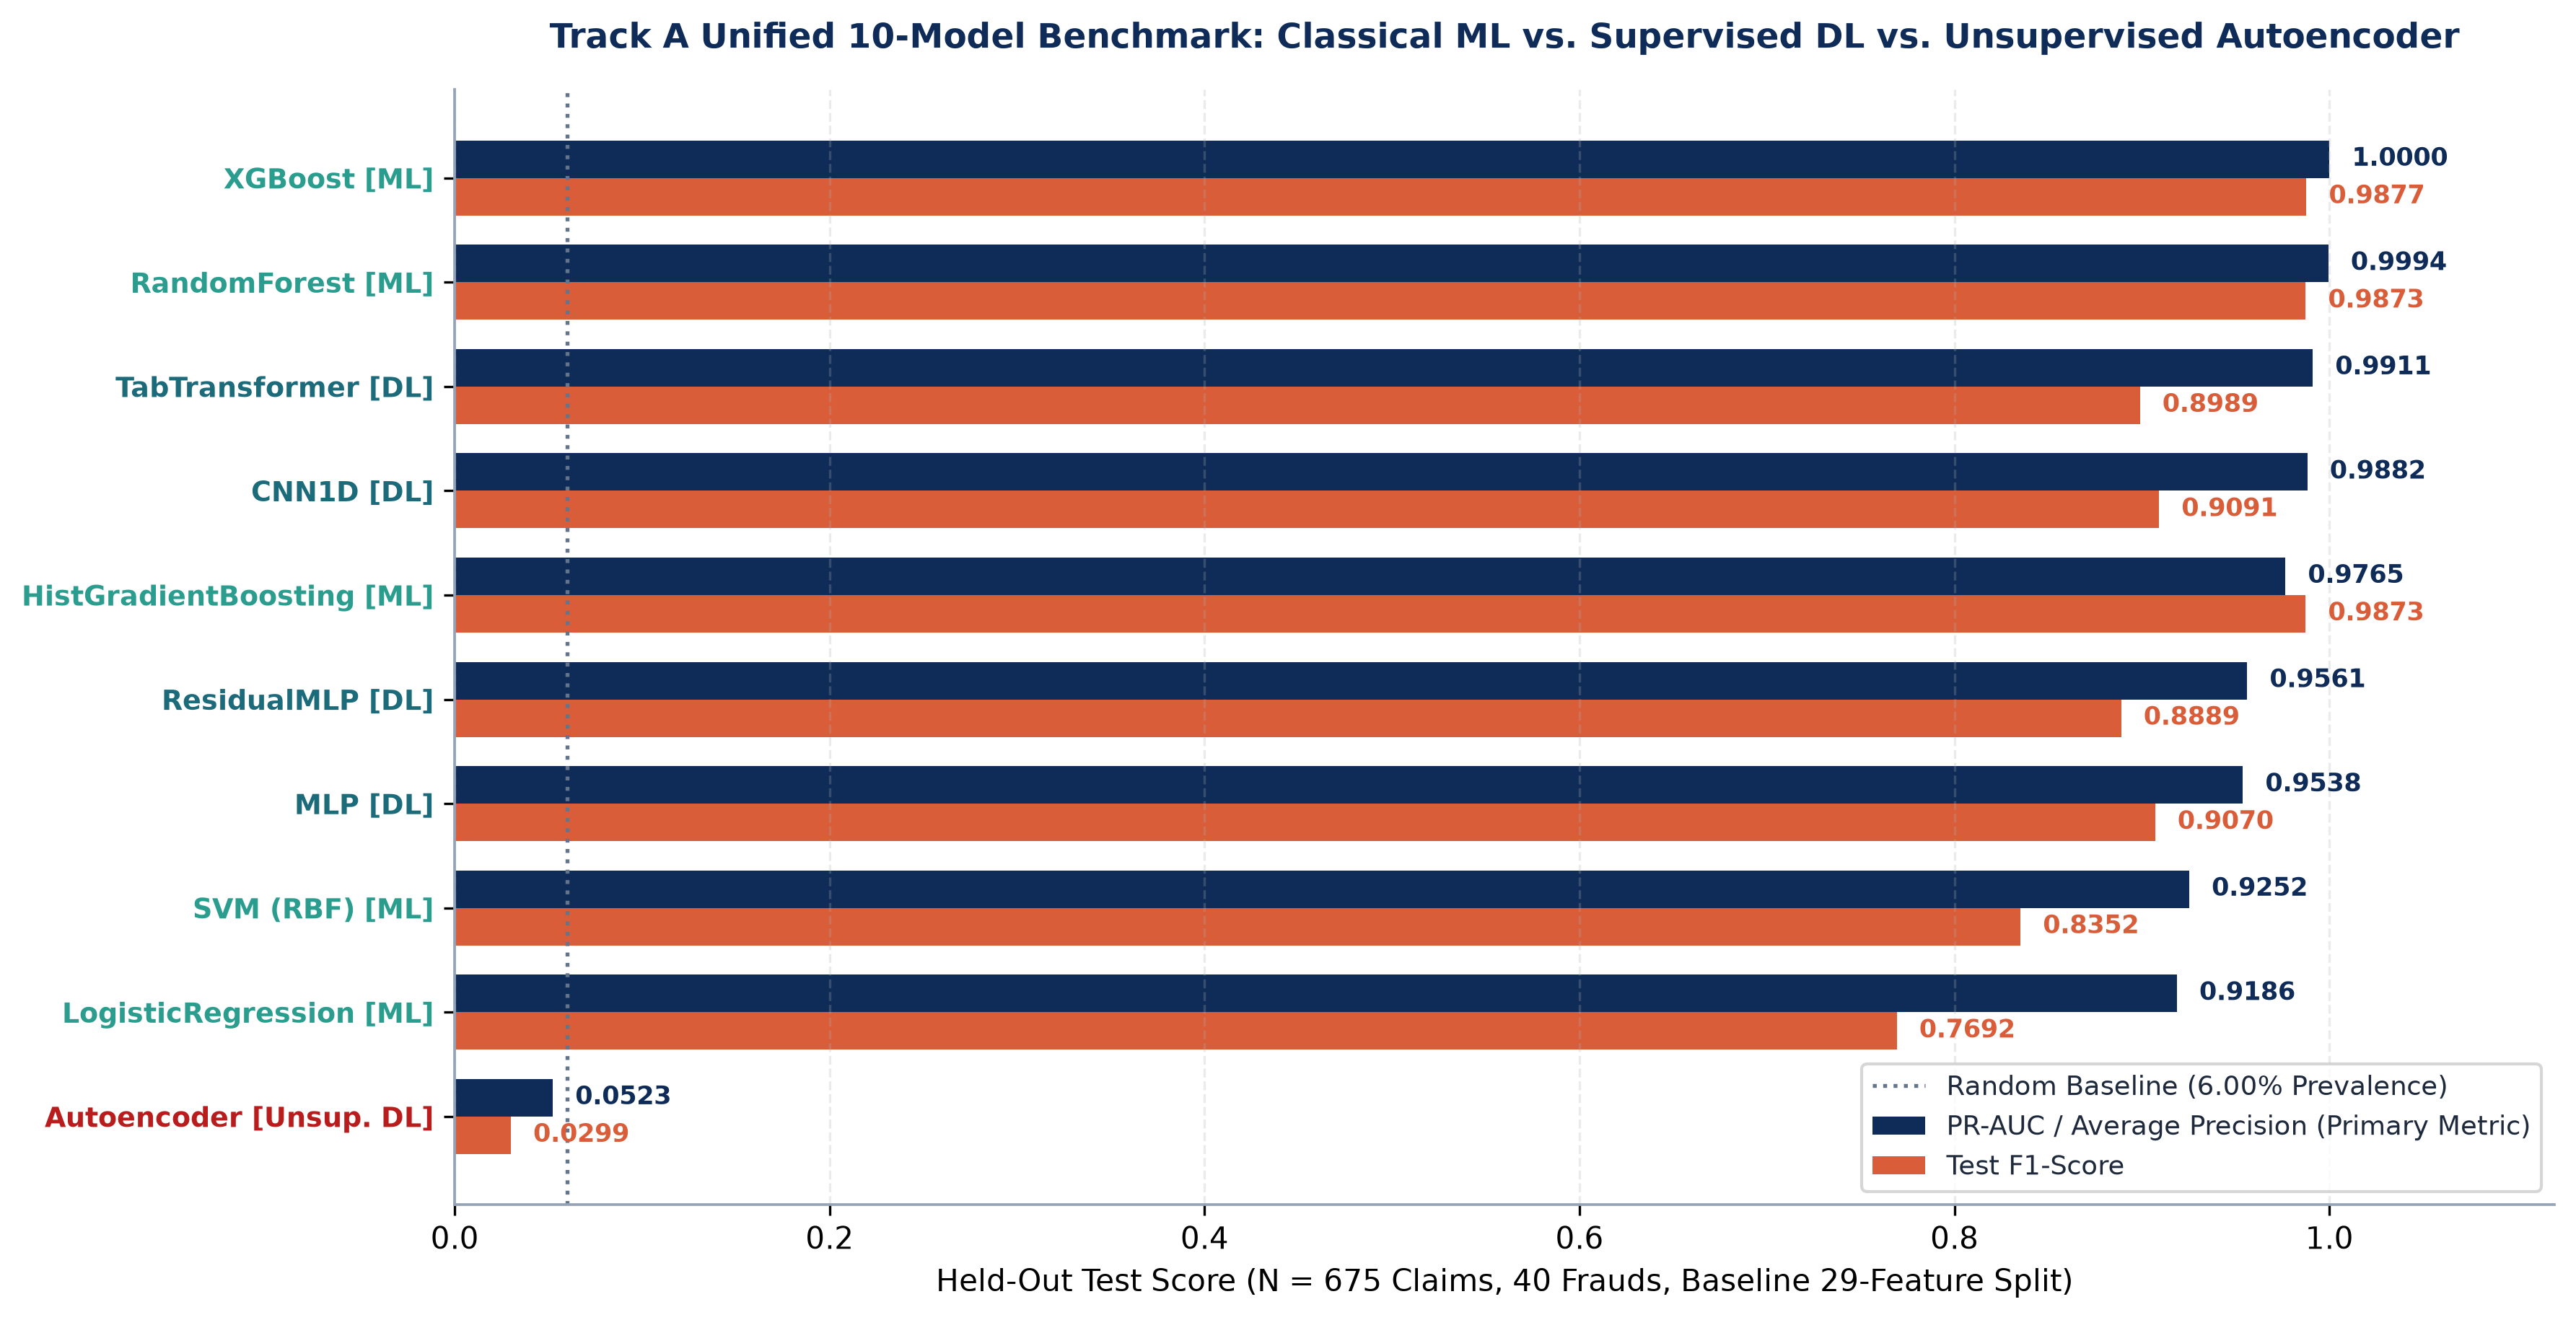
\includegraphics[width=\columnwidth]{figures/fig3_ten_model_benchmark.png}
\caption{Track A 10-model benchmark comparing Test PR-AUC vs. $F_1$ across ML, supervised DL, and the Autoencoder negative result.}
\label{fig:tracka}
\end{figure}

\subsection{Track B: Ablations, Chronological Generalization, and Error Audit}
Table~\ref{tab:trackb} and Fig.~\ref{fig:ablation} demonstrate how feature governance alters conclusions. Eliminating \texttt{Cluster} (\texttt{Intake 28f}) preserves perfect 1.0000 PR-AUC for \texttt{RandomForest} ($F_1=0.9873$, $\tau^*=0.4167$, 0 FP, 1 FN) and \texttt{XGBoost} ($F_1=0.9877$, 1 FP, 0 FN), while degrading \texttt{SVM} (0.9252 $\to$ 0.8181), \texttt{ResidualMLP} (0.9567 $\to$ 0.8765), and \texttt{MLP} (0.9538 $\to$ 0.8866). Under chronological testing ($\ge$ \texttt{2024-03-11}), all three tree ensembles reach 1.0000 PR-AUC and 1.0000 $F_1$, whereas \texttt{CNN1D} declines to 0.9172 PR-AUC ($F_1=0.8108$). Crucially, dropping \texttt{ClaimAmount} (\texttt{No-Amount 27f}) collapses all eight models uniformly to 0.1869--0.2404 PR-AUC, proving strong billing-amount dependence in this dataset.

\begin{table}[t]
\centering
\caption{Track B Test PR-AUC ($F_1$) Across Four Protocols (\texttt{validation\_f1})}
\label{tab:trackb}
\resizebox{\columnwidth}{!}{%
\begin{tabular}{@{}lcccc@{}}
\toprule
Model & Baseline (29f) & Intake (28f) & No-Amount (27f) & Temporal ($\ge$2024-03) \\ \midrule
\textbf{RandomForest} & 0.9994 (.975) & \textbf{1.0000 (.987)} & 0.2066 (.364) & \textbf{1.0000 (1.000)} \\
\textbf{XGBoost} & 1.0000 (.988) & 1.0000 (.988) & 0.2128 (.352) & 1.0000 (1.000) \\
\textbf{GradientBoosting} & 0.9765 (.987) & 0.9765 (.987) & 0.2404 (.364) & 1.0000 (1.000) \\
\textbf{CNN1D} & 0.9882 (.927) & 0.9667 (.877) & 0.2287 (.279) & 0.9172 (.811) \\
\textbf{ResidualMLP} & 0.9567 (.929) & 0.8765 (.832) & 0.2246 (.344) & 0.7979 (.723) \\
\textbf{MLP} & 0.9538 (.914) & 0.8866 (.822) & 0.2303 (.308) & 0.8581 (.696) \\
\textbf{LogisticRegression} & 0.9186 (.784) & 0.8525 (.733) & 0.2318 (.319) & 0.8799 (.740) \\
\textbf{SVM (RBF)} & 0.9252 (.897) & 0.8181 (.771) & 0.1869 (.304) & 0.8396 (.762) \\ \bottomrule
\end{tabular}%
}
\end{table}

\begin{figure}[t]
\centering
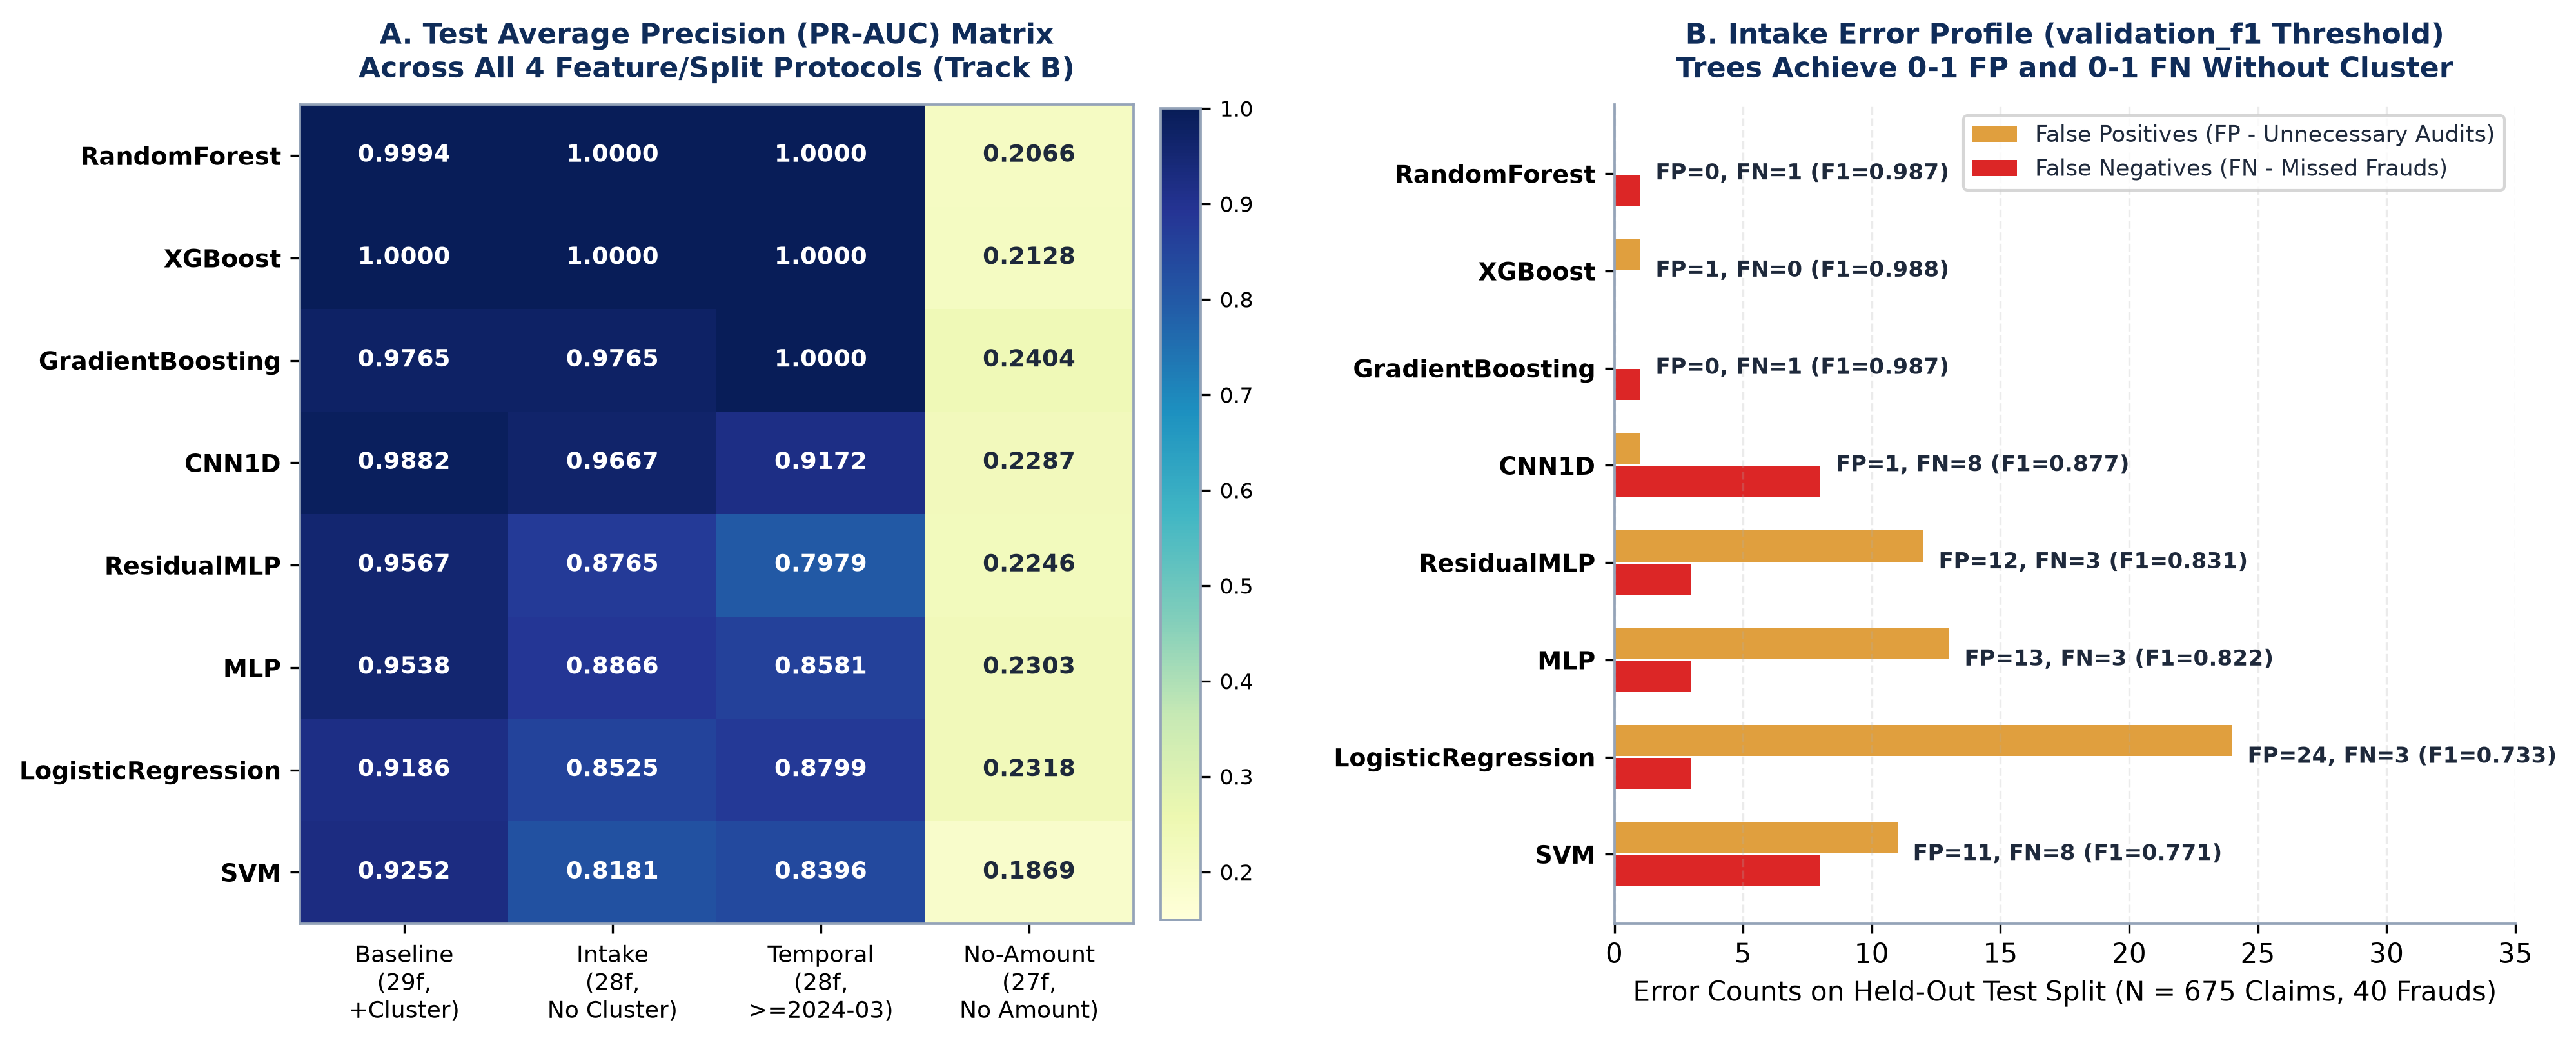
\includegraphics[width=\columnwidth]{figures/fig4_four_experiment_ablation.png}
\caption{Track B 32-run ablation matrix: (A) PR-AUC sensitivity across feature and chronological shifts; (B) Intake error comparison without \texttt{Cluster}.}
\label{fig:ablation}
\end{figure}

Inspecting the selected default champion (\texttt{Intake RandomForest}, $\tau^*=0.4167$; Fig.~\ref{fig:verif}), its single false negative across 675 test claims is source Row 1124 (\texttt{ClaimAmount}=7,465.07, lowest positive amount in the dataset; Age 39; Outpatient; score 0.2700). Stratified 1,000-replicate bootstrap CIs confirm 95\% bounds of $[0.9610, 1.0000]$ ($F_1$), $[0.9250, 1.0000]$ (Recall), and $[1.0000, 1.0000]$ (AP). Finally, automated Python-vs-Browser verification checks pass across 1,350 preprocessing rows (0 errors) and 10,800 score pairs ($4.42 \times 10^{-7}$ max absolute difference, 0 label flips).

\begin{figure}[t]
\centering
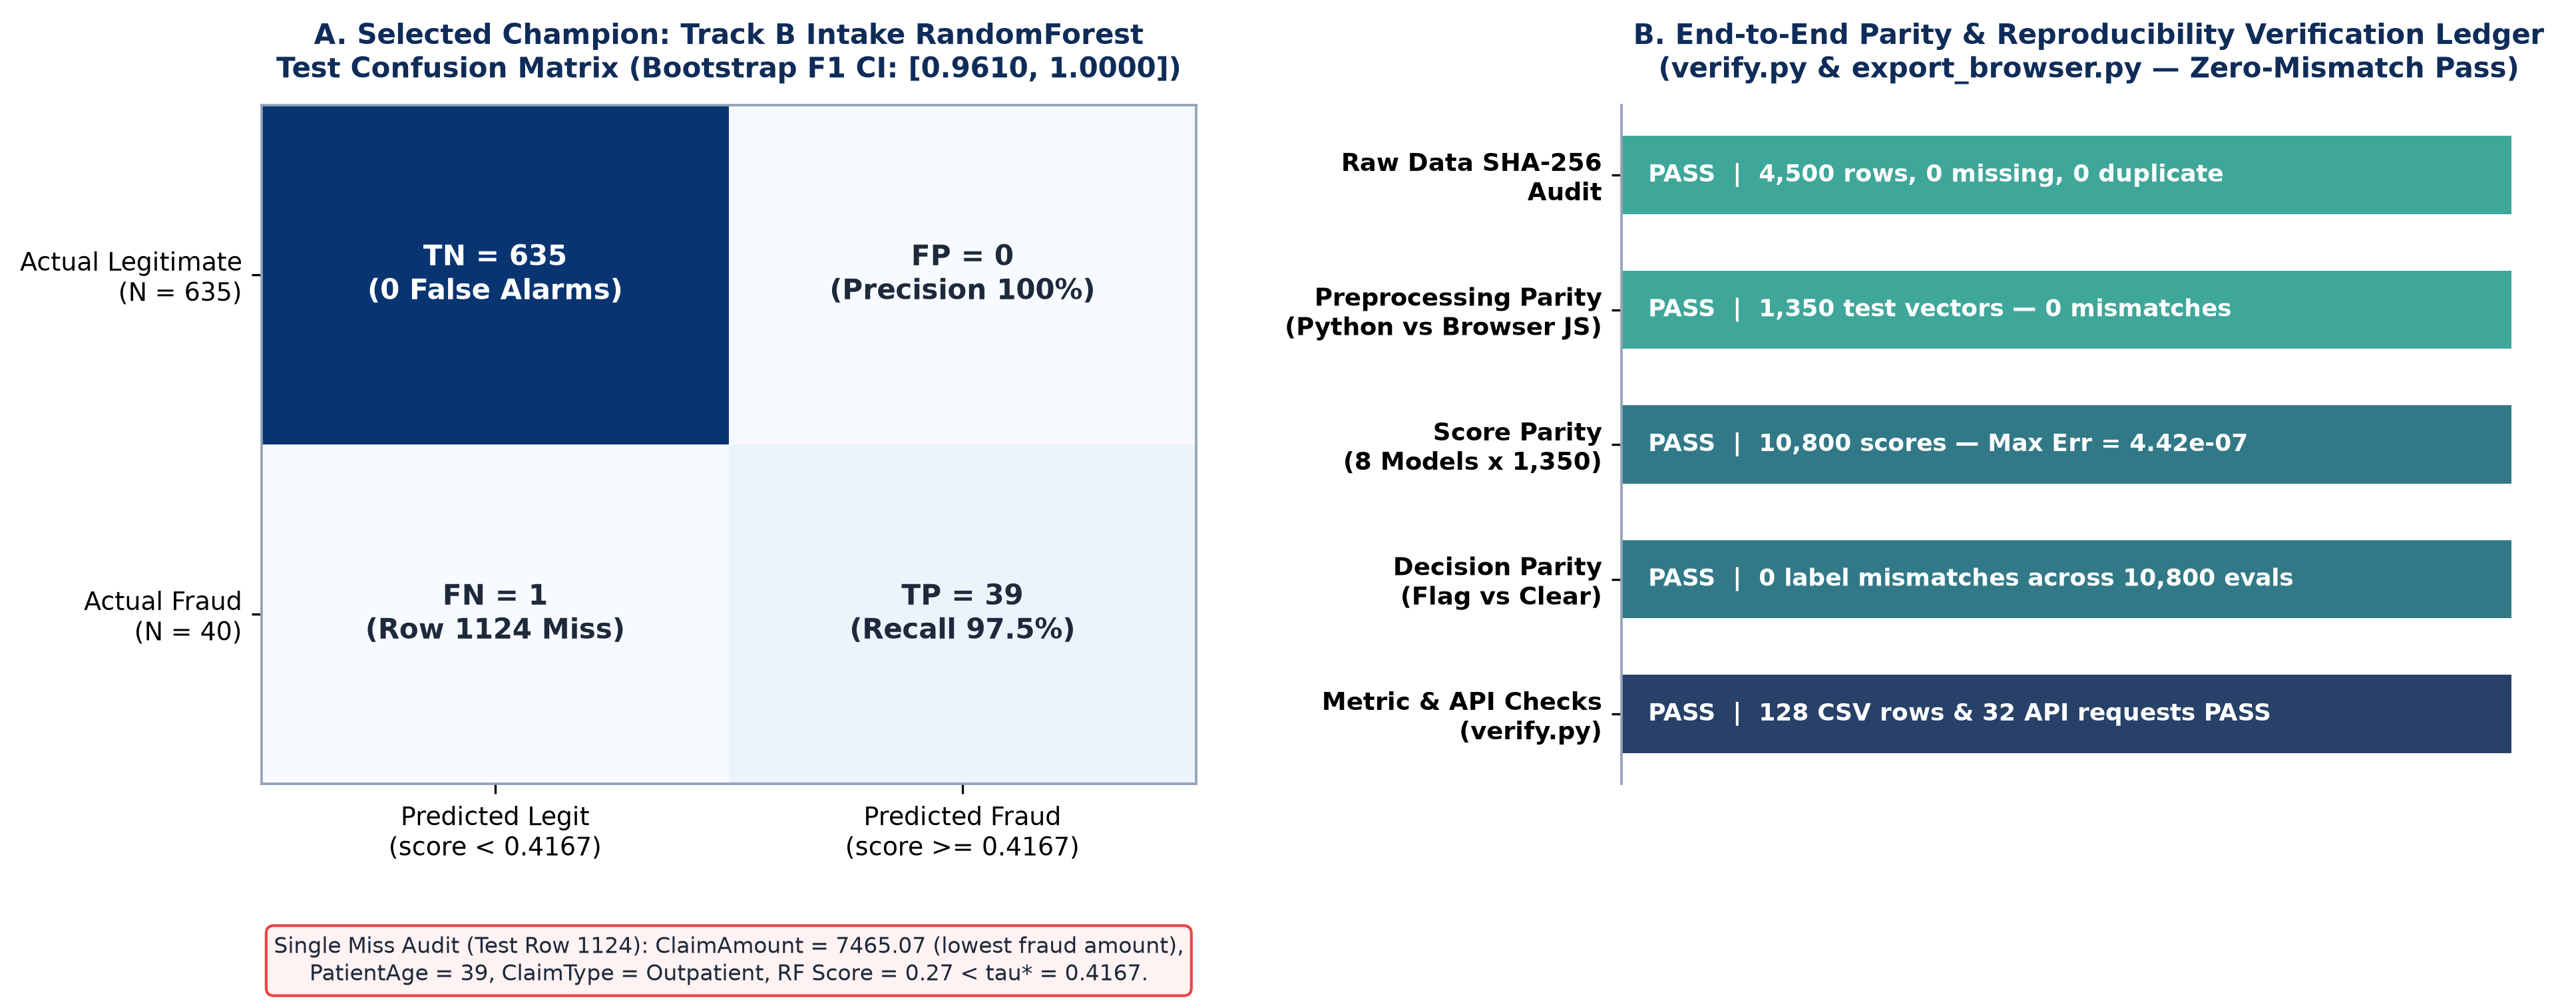
\includegraphics[width=\columnwidth]{figures/fig6_verification_and_error.png}
\caption{Selected \texttt{Intake RandomForest} confusion matrix, single-error forensic audit (Row 1124), and verified Python-to-Browser parity ledger.}
\label{fig:verif}
\end{figure}

\section{Conclusion and Future Work}
This work demonstrates that rigorous leakage governance and validation-calibrated evaluation are as decisive as classifier complexity in medical claim fraud detection. While \texttt{TabTransformer} and \texttt{CNN1D} lead neural learners, tree ensembles (\texttt{RandomForest} and \texttt{XGBoost}) outperform neural baselines reliably once spurious upstream \texttt{Cluster} labels are excluded and chronological boundaries are enforced, echoing Grinsztajn et al.\ \cite{grinsztajn2022tree}. Simultaneously, our dual-path platform validates zero-mismatch browser inference alongside full-stack FastAPI/Node/React delivery and Gemini conversational triage. Future extensions will bind Node's \texttt{/agentic/predict} directly to calibrated FastAPI model probabilities, integrate PDF/VLM OCR and policy vector RAG, and validate low-dollar upcoding detection on broader multi-institutional clinical billing corpora.

\section*{Acknowledgment}
The authors thank Prof.\ Ramesh Athe, Department of Computer Science and Engineering, IIIT Dharwad, for technical mentorship and critical experimental guidance throughout this project.

\bibliographystyle{IEEEtran}
\bibliography{references}

\end{document}
